\section{Buildroot community: support and contribution}

\begin{frame}{Documentation}
  \begin{itemize}
  \item Buildroot comes with its own documentation
  \item Pre-built versions available at
    \url{http://buildroot.org/docs.html} (PDF, HTML, text)
  \item Source code of the manual located in \code{docs/manual} in the
    Buildroot sources
    \begin{itemize}
    \item Written in {\em Asciidoc} format
    \end{itemize}
  \item The manual can be built with:
    \begin{itemize}
    \item \code{make manual}
    \item or just \code{make manual-html}, \code{make manual-pdf},
      \code{make manual-epub}, \code{make manual-text}, \code{make
        manual-split-html}
    \item A number of tools need to be installed on your machine,
      see the manual itself.
    \end{itemize}
  \end{itemize}
\end{frame}

\begin{frame}{Getting support}
  \begin{itemize}
  \item Free support
    \begin{itemize}
    \item The {\em mailing list} for e-mail discussion\\
      {\footnotesize \url{http://lists.busybox.net/mailman/listinfo/buildroot}}\\
      1300+ subscribers, quite heavy traffic.
    \item The IRC channel, {\tt \#buildroot} on the Freenode network,
      for interactive discussion\\
      130+ people, most available during European daylight hours
    \item Bug tracker\\
      \url{https://bugs.busybox.net/buglist.cgi?product=buildroot}
    \end{itemize}
  \item Commercial support
    \begin{itemize}
    \item A number of embedded Linux services companies, including
      Free Electrons, can provide commercial services around
      Buildroot.
    \end{itemize}
  \end{itemize}
\end{frame}

\begin{frame}{Tips to get free support}
  \begin{itemize}
  \item If you have a build issue to report:
    \begin{itemize}
    \item Make sure to reproduce after a \code{make clean all} cycle
    \item Include the Buildroot version, Buildroot \code{.config} that
      reproduces the issue, and last 100-200 lines of the build
      output in your report.
    \item Use {\em pastebin} sites like \code{http://code.bulix.org}
      when reporting issues over IRC.
    \end{itemize}
  \item The community will be much more likely to help you if you use
    a recent Buildroot version.
  \end{itemize}
\end{frame}

\begin{frame}{Release schedule}
  \begin{itemize}
  \item The Buildroot community publishes stable releases every three
    months.
  \item YYYY.02, YYYY.05, YYYY.08 and YYYY.11 every year.
  \item The three months cycle is split in two periods
    \begin{itemize}
    \item Two first months of active development
    \item One month of stabilization before the release
    \end{itemize}
  \item At the beginning of the stabilization phase, \code{-rc1} is
    released.
  \item Several \code{-rc} versions are published during this
    stabilization phase, until the final release.
  \item Development not completely stopped during the stabilization, a
    \code{next} branch is opened.
  \item The YYYY.02 is a long term support release, maintained during
    one year with security, bug and build fixes.
  \end{itemize}
\end{frame}

\begin{frame}{Contribution process}
  \begin{itemize}
  \item Contributions are made in the form of patches
  \item Created with \code{git} and sent by e-mail to the mailing list
    \begin{itemize}
    \item Use \code{git send-email} to avoid issues
    \item Use \code{get-developers} to know to who patches should be
      sent
    \end{itemize}
  \item The patches are reviewed, tested and discussed by the
    community
    \begin{itemize}
    \item You may be requested to modify your patches, and submit
      updated versions
    \end{itemize}
  \item Once ready, they are applied by one of the project maintainers
  \item Some contributions may be rejected if they do not fall within
    the Buildroot principles/ideas, as discussed by the community.
  \end{itemize}
\end{frame}

\begin{frame}{Patchwork}
  \begin{itemize}
  \item Tool that records all patches sent on the mailing list
  \item Allows the community to see which patches need review/testing,
    and the maintainers which patches can be applied.
  \item Everyone can create an account to manage his own patches
  \item \url{http://patchwork.buildroot.org/}
  \end{itemize}

  \begin{center}
    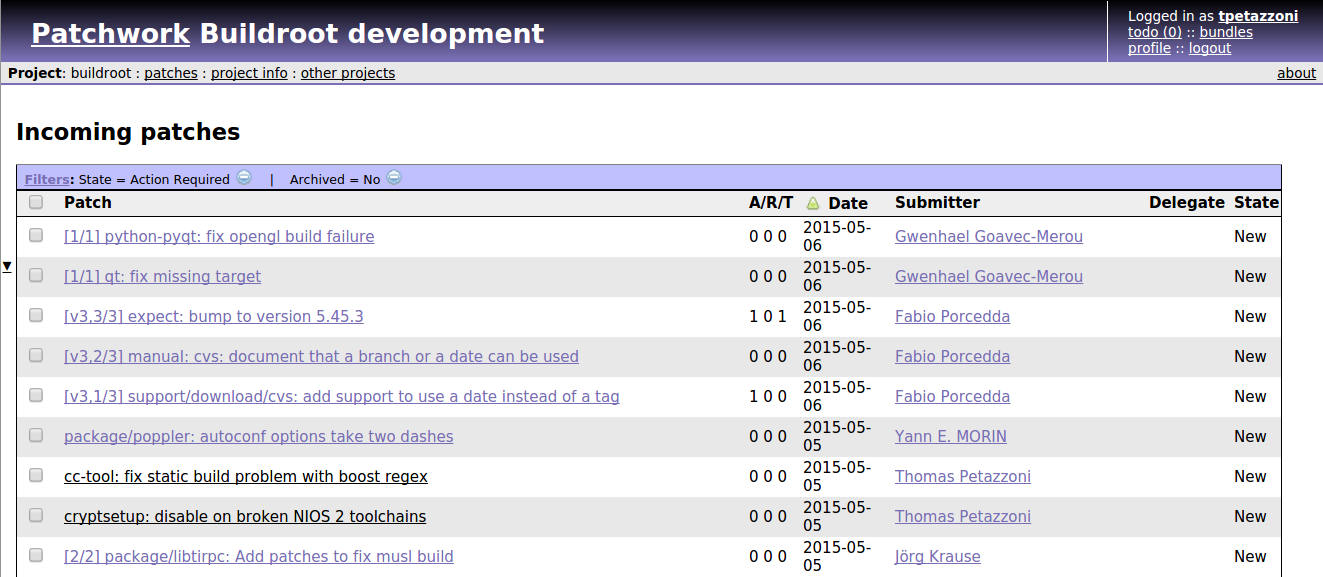
\includegraphics[width=\textwidth]{slides/buildroot-support-contribution/patchwork.png}
  \end{center}
\end{frame}

\begin{frame}{Automated build testing}
  \begin{itemize}
  \item The enormous number of configuration options in Buildroot make
    it very difficult to test all combinations.
  \item Random configurations are therefore built 24/7 by multiple
    machines.
    \begin{itemize}
    \item Random choice of architecture/toolchain combination from a
      pre-defined list
    \item Random selection of packages using \code{make
        randpackageconfig}
    \item Random enabling of features like static library only, or
      \code{BR2_ENABLE_DEBUG=y}
    \end{itemize}
  \item Scripts and tools publicly available at
    \url{http://git.buildroot.net/buildroot-test/}
  \item Results visible at \url{http://autobuild.buildroot.org/}
  \item Daily e-mails with the build results of the past day
  \end{itemize}
\end{frame}

\begin{frame}{autobuild.buildroot.org}
  \begin{center}
    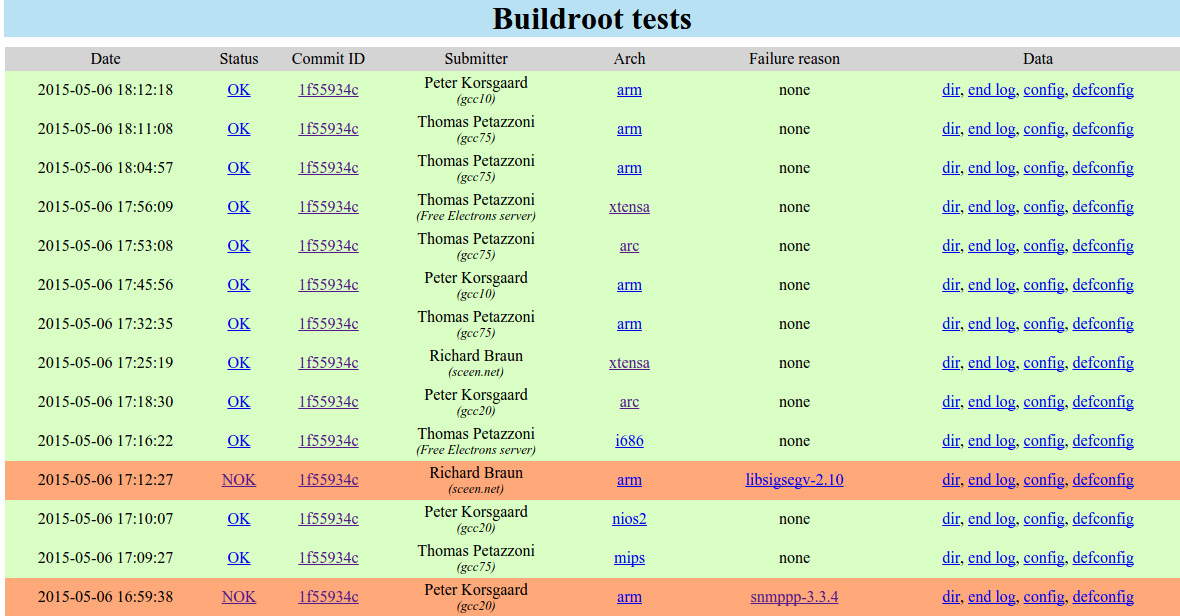
\includegraphics[width=\textwidth]{slides/buildroot-support-contribution/autobuild.png}
  \end{center}
\end{frame}

\begin{frame}[fragile]{Autobuild daily reports}

{\tiny
\begin{verbatim}
Subject: [Buildroot] [autobuild.buildroot.net] Build results for 2017-10-13
Date: Sat, 14 Oct 2017 08:30:57 +0200 (CEST)

Hello,

Build statistics for 2017-10-13
================================

      successes : 94 
       failures : 32 
       timeouts : 0  
          TOTAL : 126

Classification of failures by reason
====================================

                  dbus-1.10.24 | 13
            libtomcrypt-1.18.0 | 3 
         xkeyboard-config-2.22 | 3 
             gstreamer1-1.12.3 | 2 
[...]

Detail of failures
===================

         arc |  argp-standalone-1.3 | NOK | http://autobuild.b.n/results/bd0d198f172fa789aa2cf0bb7edb9b62a7ee247a
        m68k |         cc-tool-0.26 | NOK | http://autobuild.b.n/results/d8f0ba76f7ea1c06738658b24b8a363f8e7a526b
         arm |         dbus-1.10.24 | NOK | http://autobuild.b.n/results/ddaf58e9f8f8cfec9441ef64665e3a468b144d1f
      xtensa |         dbus-1.10.24 | NOK | http://autobuild.b.n/results/0a1e802dafd5cded6bf783127d0edbadc584583d
microblazeel |    gstreamer1-1.12.3 | NOK | http://autobuild.b.n/results/88e7208483ce1983e4f51a7e43d6877d9ff6aa66
[...]
\end{verbatim}}

\end{frame}

\begin{frame}{Additional testing effort}
  \begin{itemize}
  \item Run-time test infrastructure in \code{support/testing}
    \begin{itemize}
    \item Contains a number of test cases that verify that specific
      Buildroot configurations build correctly, and boot correctly
      under Qemu.
    \item Validates filesystem format support, specific packages, core
      Buildroot functionality.
    \item \code{./support/testing/run-tests -l}
    \item \code{./support/testing/run-tests tests.fs.test_ext.TestExt2}
    \item Run regularly on {\em Gitlab CI}
    \end{itemize}
  \item All {\em defconfigs} in \code{configs/} are built every week
    on {\em Gitlab CI}
  \end{itemize}
\end{frame}
